\documentclass[10pt, a4paper]{article}
\usepackage[a4paper,outer=1.5cm,inner=1.5cm,top=1.75cm,bottom=1.5cm]{geometry}

\twocolumn
\usepackage{graphicx}

\usepackage{hyperref}
\usepackage[utf8]{inputenc}
\usepackage{amsmath}
\usepackage{physics}
\usepackage{amssymb}
\begin{document}
\title{Assignment-4}
\author{Name:A.SUSI\and Email :  \url{susireddy9121@gmail.com}}
%\{ Wireless Communication (FWC)}
\date{30-sep-2022}
\maketitle



\section{Problem}
If three points (h, 0), (a, b) and (0, k) lie on a line, \\
$show that \frac{a}{h}+\frac{b}{k}=1$\\
\section{Solution}
\begin{center}
The input given 
\boldmath
\begin{equation} \label{eq:}
A=\begin{pmatrix} h\\ 0\ \end{pmatrix} 
\end{equation}
\begin{equation}\label{eq:}
B=\begin{pmatrix} a\\ b\ \end{pmatrix}
\end{equation}
\begin{equation}\label{eq:}
C=\begin{pmatrix} 0\\ k\ \end{pmatrix}
\end{equation}
\unboldmath
\end{center}
\begin{equation}\label{eq:}
\textbf{D=A-B}\\
=\begin{pmatrix} h\\ 0\ \end{pmatrix}- \begin{pmatrix} a\\ b\ \end{pmatrix}
\end{equation}
\begin{equation}\label{eq:}
=\begin{pmatrix} h-a\\ -b\ \end{pmatrix}\\
\end{equation}
\begin{equation}\label{eq:}
\textbf{E=A-C}\\
=\begin{pmatrix} h\\ 0\ \end{pmatrix}- \begin{pmatrix} 0\\ K\ \end{pmatrix}
\end{equation}
\begin{equation}\label{eq:}
=\begin{pmatrix} h\\ -k\ \end{pmatrix}\\
\end{equation}
\boldmath
Now the matrix is\\
\begin{equation}\label{eq:}
\textbf{F=$\begin{pmatrix} D\\ E\ \end{pmatrix}$}
\end{equation}
\unboldmath
\begin{equation} \label{eq:}
=\begin{pmatrix} h-a & -b\\ h & -k \ \end{pmatrix} 
\end{equation}

In the problem they have given that three points lie on a line, thats means these three points are collinear.\\
If  points on a line  are  collinear, rank of matrix is "1"then the vectors are in linearlydependent.\\
For 2 × 2 matrix Rank =1 means Determinant is 0.\\
Through pivoting,we obtain\\
\begin{equation}\label{eq:}
=\begin{pmatrix} h-a & -b\\ h & -k \ \end{pmatrix} \\ 
\end{equation}
\begin{equation}\label{eq:}
=\begin{pmatrix}
h-a &-b \\ 
 h& -k
\end{pmatrix}\overset{\frac{R1}{h-a}}{\rightarrow}
=\begin{pmatrix}
1 &\frac{-b}{h-a} \\ 
 h& -k
\end{pmatrix}\overset{R2\rightarrow R2-hR1}{\rightarrow}
=\begin{pmatrix}
1 &\frac{-b}{h-a} \\ 
 0&-k+\frac{bh}{h-a} 
\end{pmatrix}\\
\end{equation} 


if the rank of the matrix is 1 means any one of the row must be zero.So, making the last element in the matrix to 0.\\
\begin{equation}\label{eq:}
-k+\frac{bh}{h-a}=0
\end{equation} 
\begin{equation}\label{eq:}
(h-a)-k+bh=0\\
\end{equation} 
\begin{equation}\label{eq:}
-kh+ak+bh=0\\
\end{equation} 
\begin{equation}\label{eq:}
ak+bh=kh\\
\end{equation} 
Dividing  with kh on both sides ,we get\\

\begin{equation}\label{eq:}
\frac{a}{h}+\frac{b}{k}=1 \\
\end{equation} 

Hence proved.\\
\section{Construction}
 \begin{figure}[h]
\centering
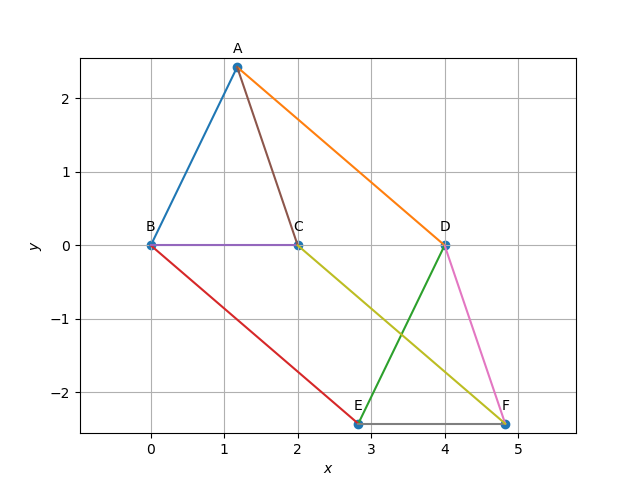
\includegraphics[scale=0.4]{fig.png} 
\caption{}
\end{figure}
\section{Code}
*Verify the above proofs in the following code.\\
\framebox{
\url{https://github.com/Susi9121/FWC/tree/main/matrix/line}}	
\bibliographystyle{ieeetr}
\end{document}
